\section{CSC Overview}
\label{sec:csc_trig}

\subsection{CSC Trigger}

Each CSC can provide up to two local charged track (LCT) segments to the trigger logic per
bunch crossing. These are formed in the trigger motherboard (TMB) and are built by combining
cathode (CLCT) and anode (ALCT) segments. The CLCT data words provide the azimuthal
position of the segment, the bend angle, and a pattern number. The ALCT data words provide
the radial position from the beamline of the segments in the chamber. The timing information
in the anode data is used to define the time of the LCT. There is one TMB, sitting in a crate on
the periphery of the detector, for each chamber. The TMB sends up to two LCTs over a custom
backplane to the muon port card (MPC).

The MPCs can receive data from up to 9 CSCs, or equivalently, can receive up to 18 LCTs.
These are sorted by rank. The best three LCTs are sent over optical fibers to the CSC Track-
Finder. There are a total of sixty peripheral crates for the CSC system, each with one MPC and
up to 9 TMBs.

The CSCTF system is partitioned into sectors that correspond to a 60$^{o}$ azimuthal region of an
endcap. Twelve “sector processors” are required for the entire system, six per endcap. Each
sector processor is a 9U VME card that is housed in a single crate. Three 1.6 Gb/s
optical links from each of five MPCs are received by each sector processor, for a total of 180
optical links for the entire system. There is no sharing of signals across neighbor boundaries,
leading to slight inefficiencies.

There are several FPGAs on each processor, but the main FPGA for the track-finding algo-
rithms is from the Xilinx Virtex-5 family. The conversion of strip and wire positions of each
track segment to ($\eta$,$\phi$) coordinates is accomplished via a set of cascaded SRAM look-up tables
(LUTs), each 512K×16 bits. These coordinates are then used for track-finding and momentum
assignment.

The CSCTF track-finding logic consists of pairwise comparisons of track segments in different
detector stations. These test for compatibility in $\phi$ and $\eta$ with a muon emanating from the col-
lision vertex within certain tolerance windows. The comparisons are then analyzed and built
into tracks consisting of possibly more than two stations. Possible duplicate (“ghost”) tracks are
canceled. The track-finding logic has the ability to accept segments in different assigned bunch
crossings by analyzing across a sliding time window of programmable length (nominally 2
BX) every bunch crossing. Duplicate tracks found on consecutive crossings are canceled. The
bunch crossing of a track is given by the second arriving track segment.

The pT of a muon candidate is calculated by using a large LUT implemented in SRAM. In-
formation such as the track type, track $\eta$, the segment $\phi$ differences between a maximum of 3
stations, and the segment bend angle in the first measurement station are used to calculate the
LUT address.

In addition to identifying muons from proton collisions, the CSCTF processors also simultane-
ously identifies any beam halo muons for monitoring and veto purposes by looking for trajec-
tories approximately parallel to the beam line.

Each CSCTF sends the up to three muon candidates each bunch crossing over a custom back-
plane to a muon sorter (MS). The MS then sorts the candidates by momentum and quality and
selects the best 4 to the GMT. The CSCTF data are also sent to a DAQ card with an SLINK
interface which puts the trigger data into the event record.

\subsection{CSC Upgrade During LS1}

During LS1, the outermost ring of the fourth disk of chambers of each endcap (ME4/2) will be
installed. This will result in four measurement stations for muons in the region 1.25 $<$ $|\eta|$ $<$
1.8 providing the additional redundancy needed in a high rate environment. For the Level-1
trigger, this coverage will improve the efficiency of the CSCTF, and improve the rate reduction
since it will be more likely to have 3 or more hits used in the pT assignment logic. No additional
hardware or reconfiguration of the present Level-1 trigger is required. The MPCs for the fourth
disk already are in place and the present CSCTF already has logic in place for these chambers.
This redundancy will extend to the more powerful algorithms envisioned for the muon trigger
upgrade as well.

The electronics for the CSC system are also under major revision. The innermost chambers of
the first endcap disks (ME1/1) provide a key sagitta measurement for the Level-1 muon trigger
in the region 1.6 $<$ $|\eta|$ $<$ 2.4. These chambers will receive new digital cathode front-end boards (DCFEB)
as well as new trigger and data acquisition electronics that will significantly enhance their
performance in the trigger and in offline reconstruction. The strips of the ME1/1 chambers are
split into two regions at $|\eta|$ = 2.1. The high region $|\eta|$ $>$ 2.1 currently has strips triple-ganged
in the electronics for both the trigger and readout, making it ambiguous as to which third of
the chamber generated a particular hit (the ganging has every 16th strip ganged to each other, 
where there are 48 strips in total across a chamber layer). The ambiguity can be mitigated using measurements
from the outer stations. The pT resolution using only the outer stations is quite coarse, leading
to a significantly increased single muon trigger rate in the region 2.1 $<$ $|\eta|$ $<$ 2.4. The region
2.1 $<$ $|\eta|$ $<$ 2.4 currently generates a single muon trigger rate comparable to that of the entire
region $|\eta|$ $<$ 2.1. With the new digital front-end boards and Trigger Motherboards (TMBs),
this triple-ganging will be removed, leading to much improved triggering for $|\eta|$ $>$ 2.1. This
should allow CMS to maintain full muon trigger coverage to $|\eta|$ = 2.4 after LS1. The recovered
older electronics will be used to instrument the new ME4/2 chambers.

\begin{figure}[t]
        \begin{center}
                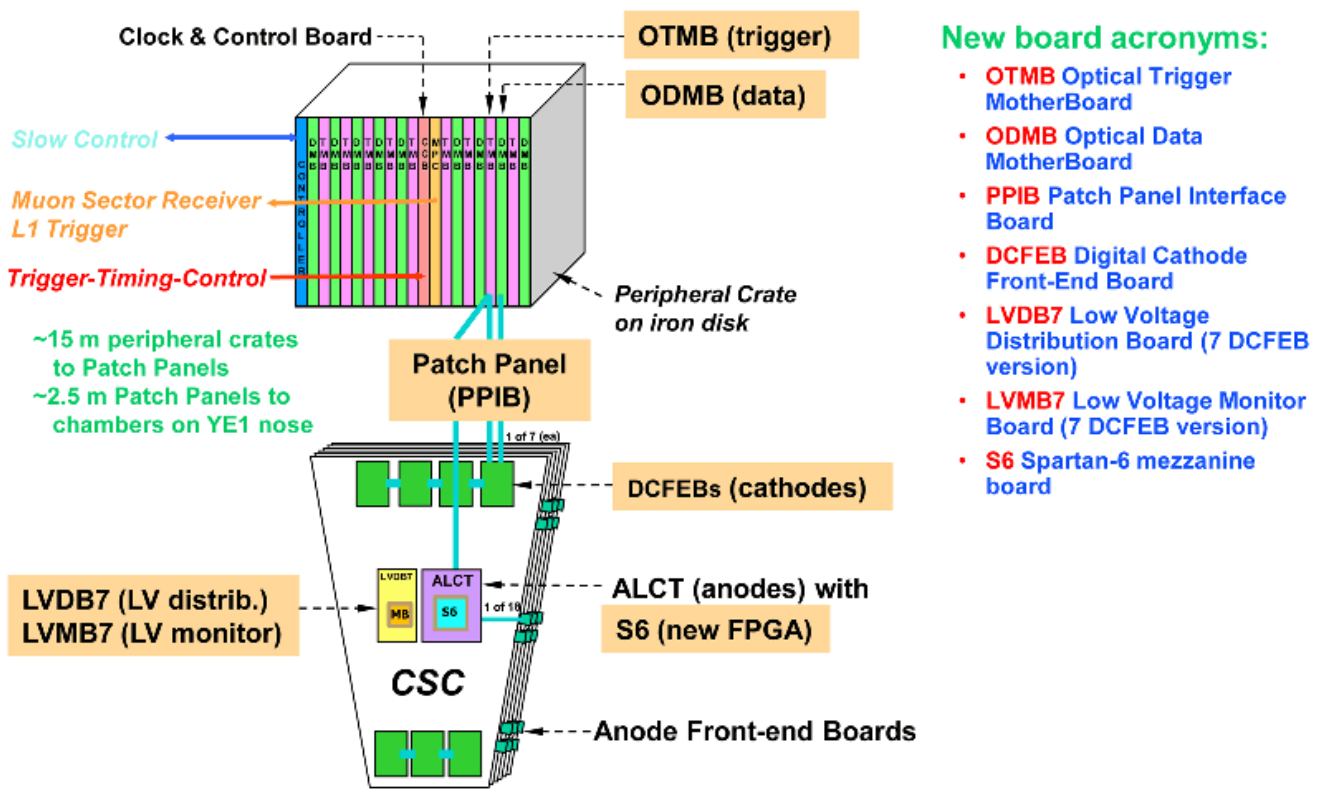
\includegraphics[width=0.90\linewidth]{figures/ME11_upgrade_overview.png}
                \caption{Schematic overview of the ME1/1 chambers upgrade.}
                \label{fig:me11_upgrade_overview}
        \end{center}
\end{figure}

\begin{figure}[t]
        \begin{center}
                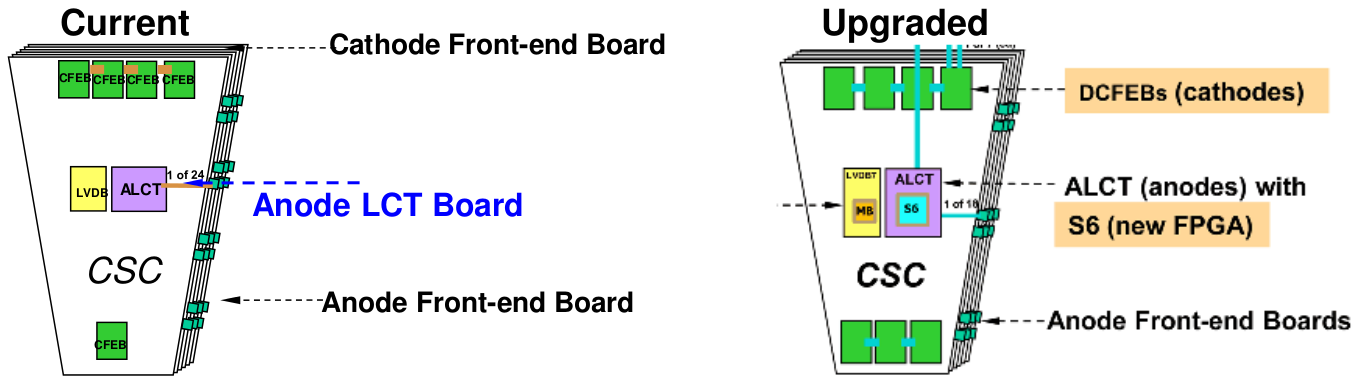
\includegraphics[width=0.90\linewidth]{figures/ME11_upgrade_electronics.png}
                \caption{Schematic overview of the ME1/1 electronics upgrade.}
                \label{fig:me11_upgrade_electronics}
        \end{center}
\end{figure}